\documentclass[11pt]{article}
\usepackage[utf8]{inputenc}
\usepackage{lmodern}
\usepackage[T1]{fontenc}
\usepackage{float}
\usepackage{hyperref}
\usepackage{graphicx}
\usepackage{amsfonts}
\usepackage[rightcaption]{sidecap}

\hypersetup{
  % parametrage des hyperliens
  colorlinks = true, % colorise les liens
  breaklinks = true, % permet les retours à la ligne pour les liens trop longs
  linkcolor = black, % couleur des liens internes aux documents
  citecolor = black, % couleur des liens vers les references bibliographiques
  urlcolor = blue, % couleur des hyperliens
}
\begin{document}

\title{Bilan du Projet S3}
\author{Arthur Correnson}
\maketitle

\section*{Introduction}

Lors du semestre 3 de licence, il nous a été demandé d'implémenter en langage C un logiciel de résolution du \textbf{problème du voyageur de commerce}. Ce problème d'optimisation combinatoire est insoluble en grande dimension, mais plusieurs méthodes permettent d'approcher la solution optimale à moindre coût. Nous proposons ici quatre méthodes de résolution :

\begin{itemize}
	\item \textbf{Force Brute} 	Recherche exhaustive du plus court chemin.
	\item \textbf{Algorithme génétique} 	Approche évolutive basée sur le croisement de solutions intermédiaires.
	\item \textbf{Plus Proche voisin}	 	Méthode heuristique calculant de proche en proche le plus court chemin.
	\item \textbf{Marche aléatoire} Tirage au sort d'un chemin.
\end{itemize}

Notons qu'une méthode d'optimisation nommée \textbf{2 optimisation} a aussi été développée. Elle permet d'améliorer les résultats obtenus par les méthodes précédentes.

\section*{Programme rendu}

La réponse au sujet prend la forme d'un programme C utilisable en ligne de commande. Il attend en entrée un fichier au format standard \href{http://comopt.ifi.uni-heidelberg.de/software/TSPLIB95/}{TSP} décrivant le problème à résoudre et produit une solution au problème sous la forme d'un fichier \textbf{CSV}. Les quatre méthodes demandées ont été implémentées et vérifiée.

\subsection*{Structure des sources}

Le code source est organisé selon une arborescence stricte :

\begin{itemize}
	\item 	\textbf{docs/} : La documentation
	\item 	\textbf{scripts/} : Scripts utiles python (affichage graphique des résultats)
	\item 	\textbf{data/} : Exemples de fichiers TSP et des résultats associés.
    	\item 	\textbf{src/} : contient le code source en C
    \item 	\textbf{src/tsplib/} : module d'interaction avec les fichiers au format TSP.
	\item	\textbf{src/methods/} : implémentation des différentes méthodes de résolution
   	\item 	\textbf{include/} : contient tous les en-têtes
   	\item	\textbf{include/tsplib} : en-têtes pour le module tsplib
	\item 	\textbf{include/methods} : en-têtes pour le méthodes de résolution
    \item 	\textbf{tests/} : dossier contenant les modules de tests unitaires.
\end{itemize}

Notons que la séparation des sources et des en-têtes est un choix de design utilisé afin de faciliter l'usage de notre programme à la fois en tant que logicielle, mais également en tant que bibliothèque utilitaire. Le programmeur souhaitant re-exploiter tout ou partie de ces sources pourra aisément importer les en-têtes de son choix en passant l'option -I include/ au compilateur C.

\subsection*{Compilation}

Le \textit{pipeline} de compilation a été écris en \href{https://cmake.org}{CMake}, une alternative aux \textit{Makefiles}, par soucis de clarté et de simplicité. Un \textit{Makefile} principale placé à la racine permet cependant de contrôler toutes les tâches liées au projet. \\

\begin{tabular}{ | l | l | }
	\textbf{commande}	& \textbf{utilisation} \\
	make build 	& compilation de l'ensemble des sources \\
	make run 		& lance le programme sur un petit exemple  \\
	make graph & affichage graphique des résultats de tests \\
	make doc		& génère la documentation avec Doxygen \\
	make clean 	& Nettoie le dossier de build et les artefacts de compilation \\
\end{tabular}

\subsection*{Utilisation du programme}

\begin{tabular}{ | c | l | }
	\textbf{option}	& \textbf{méthode} \\
	-bf		& Force Brute \\
	-bfm	& Force Brute (optimisation matricielle) \\
	-ga		& algorithme génétique \\
	-rw		& marche aléatoire (\textit{Random Walk}) \\
	-ppv		& plus proche voisin (\textit{Nearest Neighbour}) \\
	-2opt 	& application de la \textbf{2-optimisation} \\
\end{tabular}

\section*{Points Forts du Projets}

Au cours du développement du projet, l'accent à été mis sur plusieurs points. En particulier, une grande importance a été accordée à la \textbf{fiabilité}, la \textbf{généricité}, la \textbf{maintenabilité}, la \textbf{documentation} ainsi que la qualité des \textbf{entrées/sorties}.

\subsection*{Fiabilité}

Certains algorithmes (ou portion d'algorithmes) de résolution du problème du voyageur de commerce sont assez délicats, de leur bonne implémentation dépend la qualité des résultats obtenus ou même la terminaison du programme. Aussi, les portions les plus complexes d'algorithmes ont été développée avec le soucis d'être correcte et vérifiée. Cette vérification passe par des tests unitaires, mais également par l'utilisation d'assertions. Par ailleurs, les algorithmes ont été travaillé manuellement avant d'être implémenté dans une version en langage C. Parmi les portions vérifiées du programme, on trouve \textbf{l'algorithme de calcul des permutations} utilisée pour la méthode Force Brute (la preuve a été faite manuellement), et l'algorithme de \textbf{croisement DPX} utilisé pour l'algorithme génétique. De même, la cohérence de l'ensemble des méthodes de résolutions a été testée sur des jeux d'exemples (notamment, la vérifications que les réponses obtenus sont bien des permutations).

\subsection*{Généricité}

Une mauvaise utilisation du programme ou le nom respect des formats de données ne doit pas causer le plantage du programme. Aussi, la lecture des entrées a fait l'objet d'un traitement exhaustif. Un \textit{parser} complet a été implémenté pour lire les paramètres de la ligne de commande ainsi que les fichiers \textbf{TSP}. En cas de non respect des formats, un message d'erreur précis est affiché. 

\begin{figure}[H]
	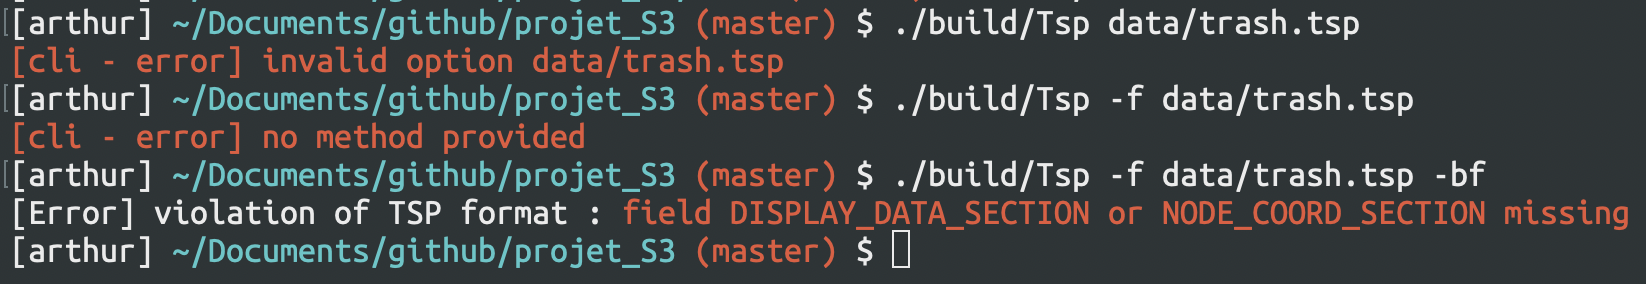
\includegraphics[scale=0.5]{capture.png}
\end{figure}

\subsection*{Maintenabilité}

La maintenabilité est la facilité d'un projet à être administré, modifié, corrigé et partagé. Ici, le code source a été écris avec une attention particulière portée à la clarté et à la lisibilité du code. Ainsi, il est relativement aisé de se plonger dans la compréhension du code source et donc d'appliquer des éventuels correctifs ou modifications. De plus, un formateur de code a été utilisé pour s'assurer que le code satisfait à des standards strictes en terme de disposition et de lisibilité.

\subsection*{Entrées/sorties}

La qualité des entrées sorties est une chose très importante. Le logiciel demandé s'utilise en ligne de commande, l'absence de retour graphique implique donc un soin d'autant plus grand des interactions avec l'utilisateur (puisque pas d'interface graphique). Aussi, les informations affichées par le programme sont formatées et misent en couleur. C'est un détails simple à mettre en place mais qui améliore grandement l'expérience utilisateur. De plus, un script d'affichage graphique des solutions est fournis avec le programme. Cela permet de visualiser les résultats produits par le logiciel.

\begin{figure}[H]
	\centering
		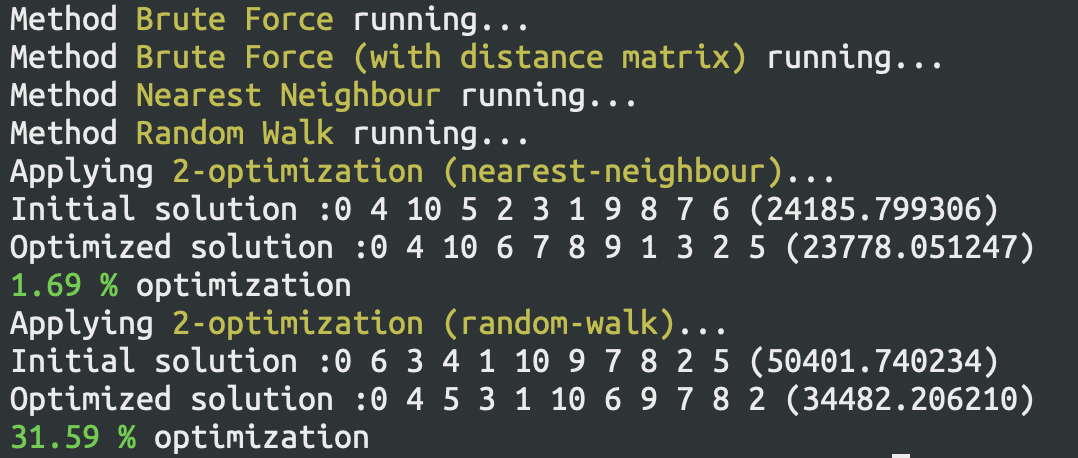
\includegraphics[scale=0.5]{capture_2} \\
\end{figure}
\begin{figure}[H]
	\centering
		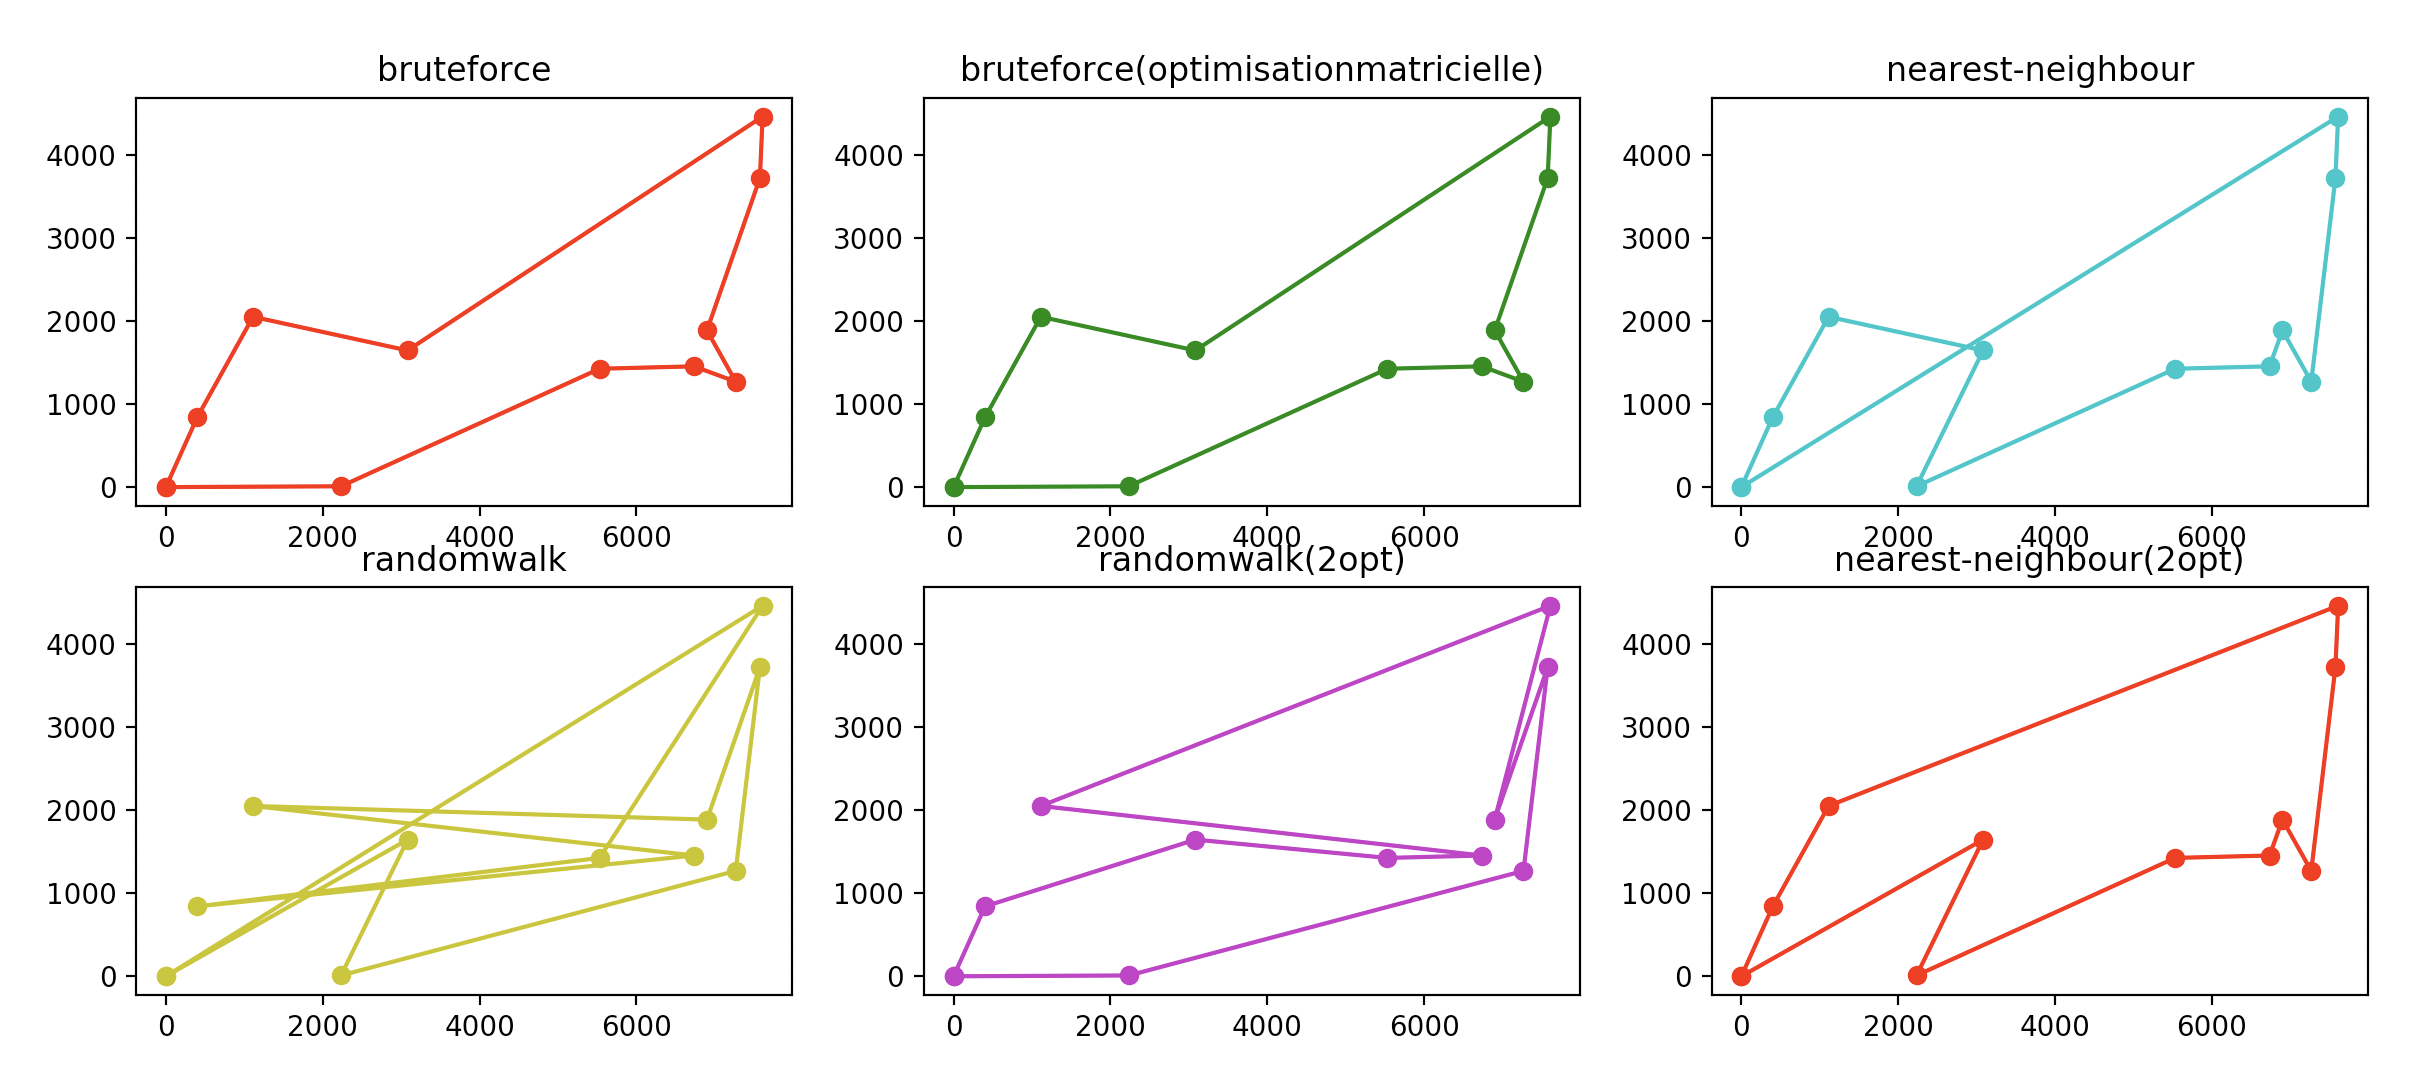
\includegraphics[scale=0.25]{capture_3} \\
\end{figure}


\subsection*{Résultats}

Les résultats obtenus sur les problèmes \textbf{att10}, \textbf{att20} et \textbf{att48} (trois problèmes de la bibliothèque TSPLIB) sont convaincants. La méthode génétique est de loin la meilleure, elle donne les plus petites longueurs en comparaison avec les approches \textbf{Plus Proche Voisin} et \textbf{Marche Aléatoire}.\\

\begin{tabular}{ | c | c | c | c | }
	\textbf{problème} & \textbf{plus proche voisin + optimisation} & \textbf{génétique} \\
	att10	& 23778.05 & 21088.99 \\
	att20	& 26634.01 & 24113.94 \\
	att48	& 42084.34 & 39719.07 \\
\end{tabular}

\subsection*{Conclusion}



\end{document}